%%%%%%%%%%%%%%%%%%%%%%%%%%%%%%%%%%%%%%%%%%%%%%%%%%%%%%%%%%%%%%%%%%%%%%%%%%%%%%%%
%%  METHODOLOGY
%%%%%%%%%%%%%%%%%%%%%%%%%%%%%%%%%%%%%%%%%%%%%%%%%%%%%%%%%%%%%%%%%%%%%%%%%%%%%%%%
\chapter{Methodology}\label{methodology}
We build the system around a single idea: natural-language task planning can be both flexible and reliable if a locally hosted \gls{vlm} is grounded in a structured pool of basic operations and retrieves them on demand. The same grounded vocabulary carries over to cooperation, allowing the model to compose dual-arm coordination at runtime rather than following a hard-coded joint path. Everything else builds on this core. The reflection strategy adds recovery, while the \gls{kg}, the \gls{vgn} grasping backend, the negotiation protocol, and the AutoRT adaptation function as optional extensions that broaden the system’s capabilities.

We begin with the operations system and supporting infrastructure, then move to the task planning pipeline, our main contribution, and close with the coordination mechanisms that extend single-robot behavior to collaborative multi-robot tasks.

% ------------------------------------------------------------------------------
\section{System Architecture Overview}\label{sec:overview}
Two pieces of infrastructure support everything else: a Python stack with \gls{ros}~\cite{Macenski_2022}/\allowbreak MoveIt~\cite{coleman2014reducingbarrierentrycomplex} for motion planning, and a Unity simulation for physics and execution. We chose Unity mostly for continuity, as we build on the existing RoboScan project~\cite{roboscan}, which already provided a Unity-based simulation foundation for the AR4~\cite{AnninRobotics2026} arms. Unity’s editor also makes it easy to build and iterate on scenes with multiple robot instances and objects, and its \texttt{ArticulationBody} physics component can handle the AR4’s six-joint kinematics. We considered alternatives such as Gazebo~\cite{gazebo}, but Apple Silicon compatibility issues ruled it out early in development. Figure~\ref{fig:system_overview} shows how the pieces fit into the four-layer architecture described in the rest of this chapter.

\begin{figure}
	\centering
	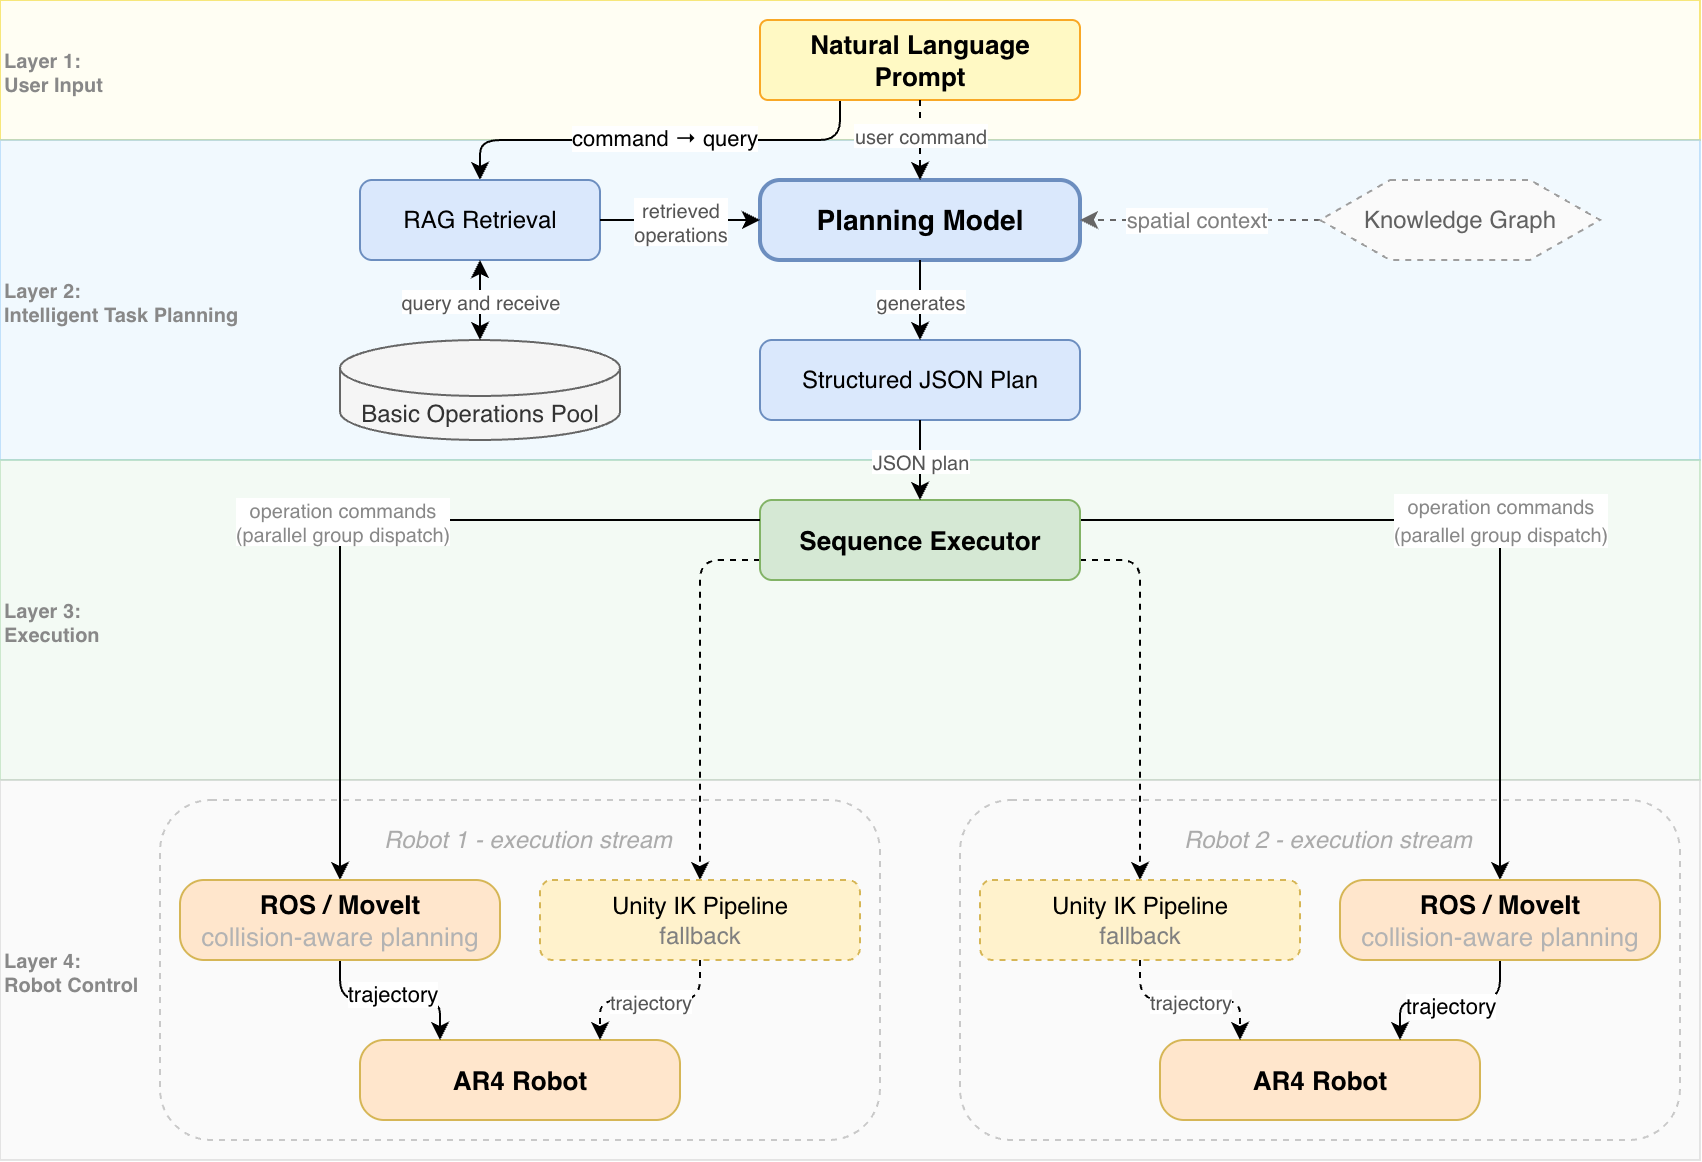
\includegraphics[width=1.0\linewidth]{images/16_system_flow.png}
	\caption{Simplified system architecture overview showing how a natural language prompt flows through the system’s four layers. Layer 1 accepts the user command and passes it to the planning layer. Layer 2 retrieves semantically relevant operations from the basic operations pool via \gls{rag}, sends them to the model, and receives a structured JSON plan. Layer 3 dispatches the plan through the sequence executor, coordinating the two robots via signal/wait synchronization and, where needed, parallel group dispatch. Layer 4 executes the resulting operation commands on the two AR4 arms through either \gls{ros}/MoveIt as a collision-aware planning backend, or the Unity \gls{ik} pipeline (dashed). The \gls{kg} provides optional spatial context to the planning layer.}
	\label{fig:system_overview}
\end{figure}

\subsection{Operations System}\label{sec:operations}
The operations system is the vocabulary the command pipeline uses. Each operation is a self-contained unit with a name, a typed parameter schema, and a structured result format. The two orthogonal axes, function and complexity level, classify them (Figure~\ref{fig:operation_map}). Below, we focus on the complexity axis because it supports failure diagnosis and tracks task difficulty. We considered a flat list, which is simplest but sacrifices failure diagnosis, and a dependency graph, which is more precise but adds complexity without practical benefit at the model-facing API level, where operations are selected by semantic intent. The level hierarchy preserves the same structural information in a form immediately useful to developers. We chose four levels because they align with real architectural boundaries:

\begin{description}
	\item[Atomic] covers single, indivisible commands with no perception dependencies and serves as a building block for higher levels.
	\item[Basic] covers simple coordinated actions that dispatch a single command and return immediately, while introducing perception, such as field detection and point-cloud generation. These also serve as building blocks for higher-level operations.
	\item[Intermediate] covers composite operations spanning object-level perception, spatial navigation, and manipulation. Its manipulation and navigation members internally invoke atomic and basic operations.
	\item[Complex] covers the task-level operations: the heaviest single-call compositions, each bundling a full perception–plan–execute pipeline for one arm, such as the grasp pipeline and the receive side of an inter-robot handoff.
\end{description}

The levels correspond to the evaluation benchmarks defined in Section~\ref{sec:benchmark-framework}. Tasks of increasing difficulty progressively exercise higher levels of the system. The practical benefit is failure diagnosis. If a Complex task fails, the developer can verify that the constituent lower-level operations succeed in isolation before investigating the composition logic. In total 20 operations are registered at startup across the four levels.

\begin{figure}
	\centering
	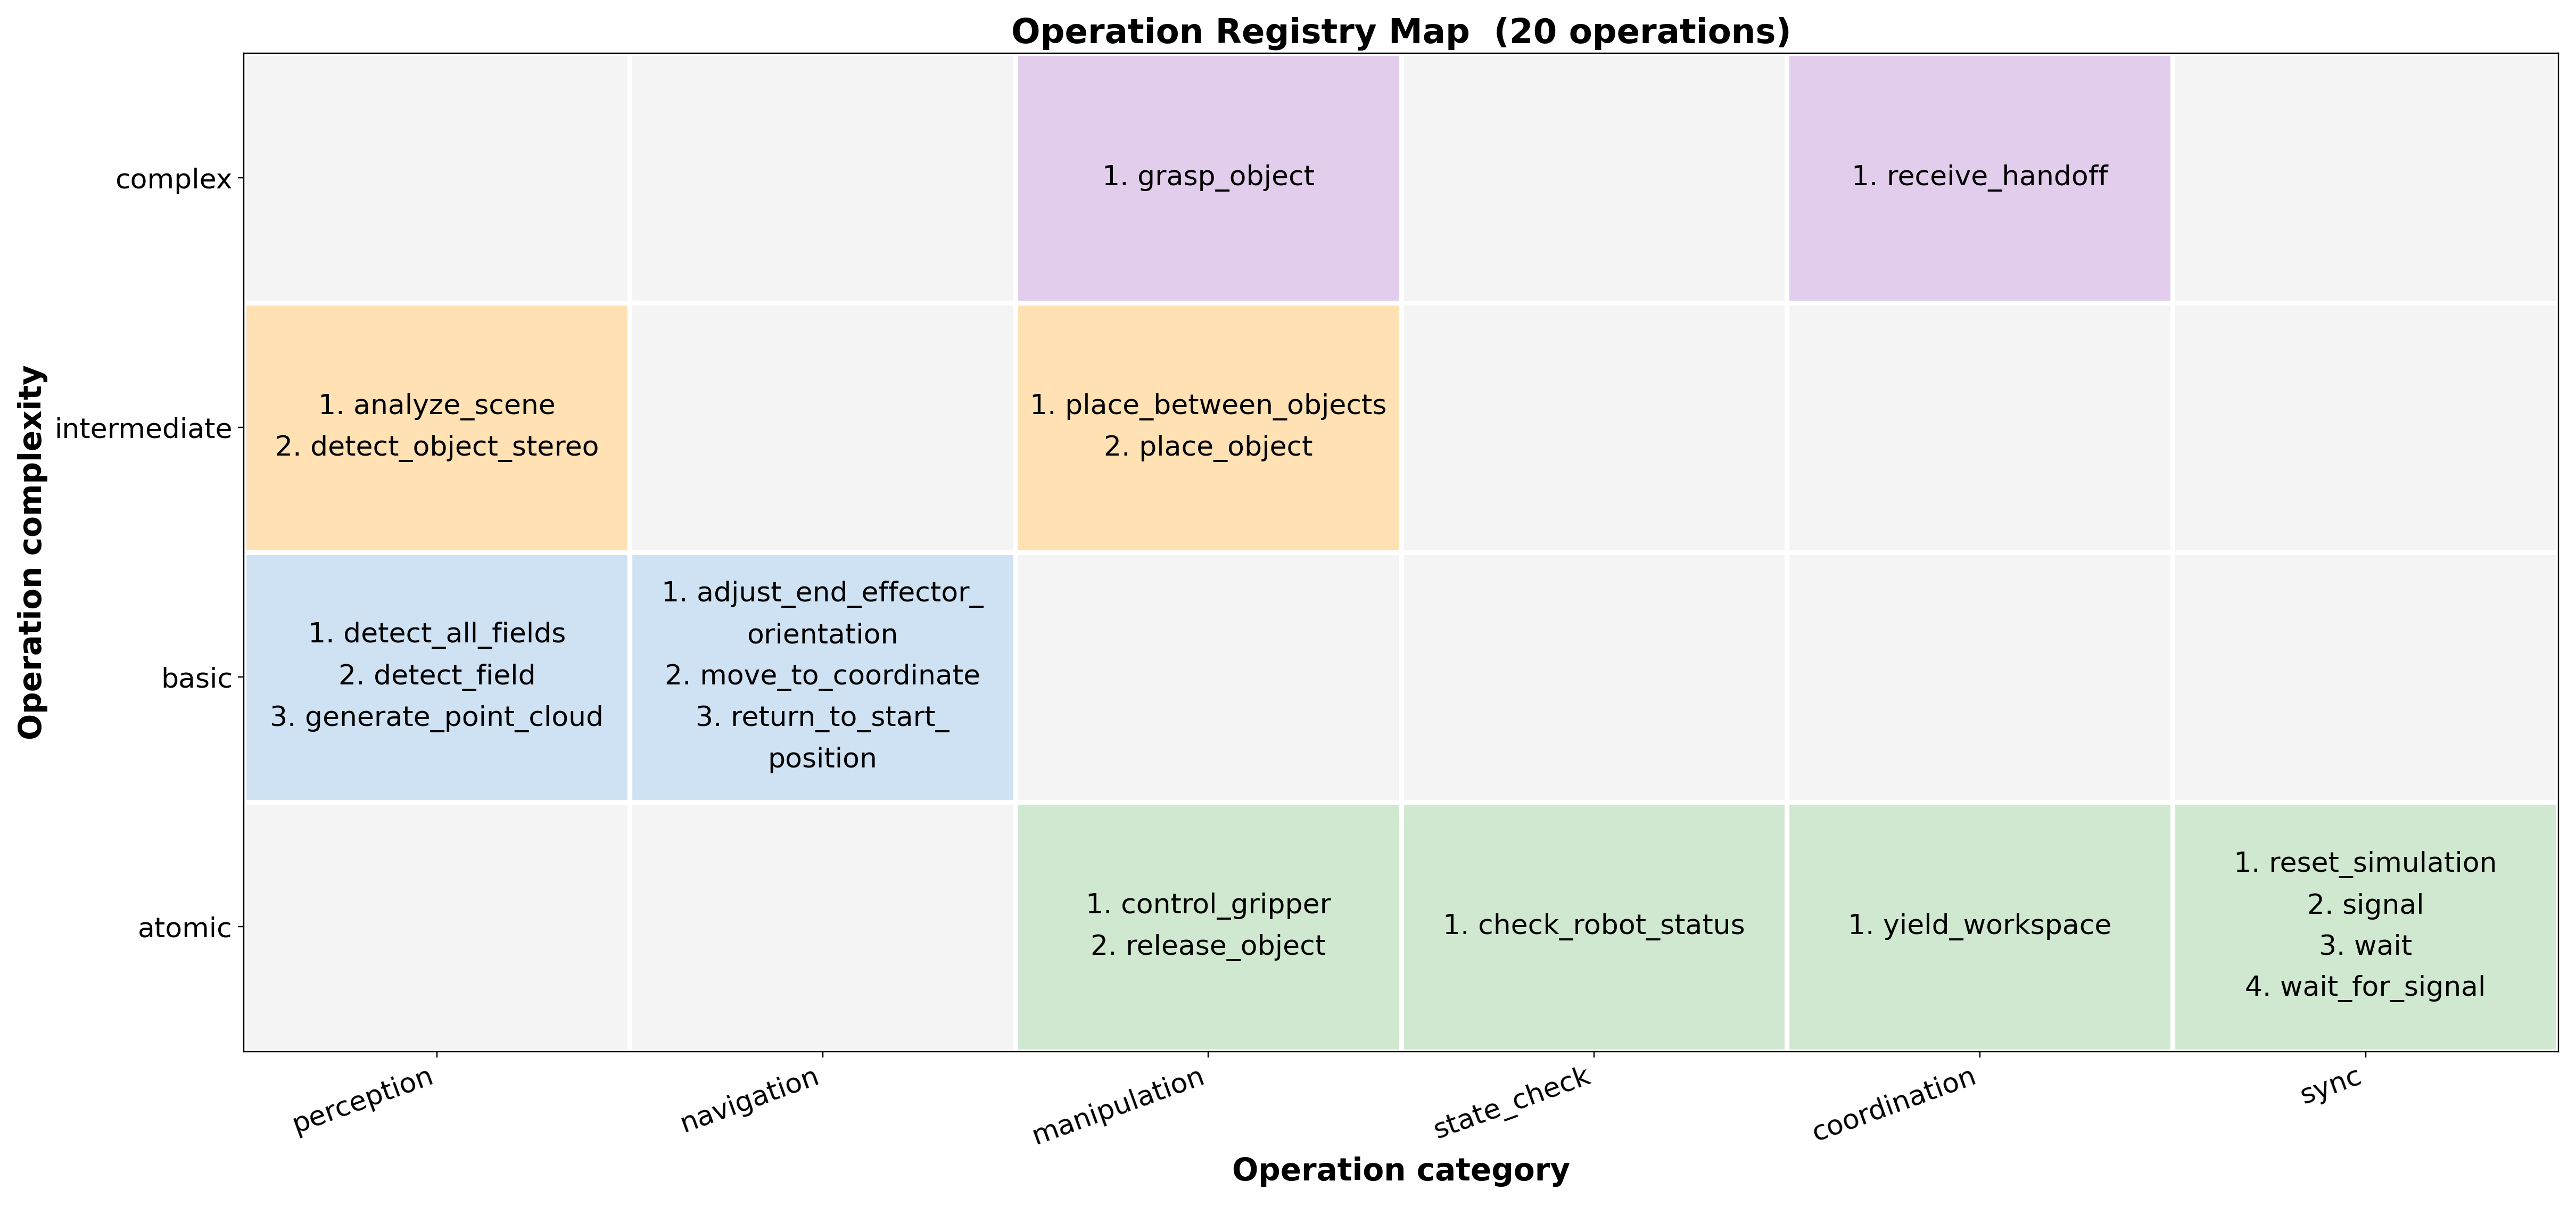
\includegraphics[width=1.0\linewidth]{images/09_operation_map.png}
	\caption{Operation registry map. The 20 operations are arranged by complexity and category.}
	\label{fig:operation_map}
\end{figure}

\subsection{Robot Operating System}\label{sec:ros}
We integrate MoveIt only as a planning backend, not as a full robot controller. This way, path computation and physical execution stay separate. MoveIt computes joint trajectories, and Unity executes them through its \texttt{ArticulationBody} physics engine. This split keeps the simulation as the single authoritative source for the robot state and eliminates the need for a \gls{ros} hardware interface or fake driver in the \gls{ros} stack. The backend is selectable at runtime depending on whether collision-aware planning is needed; Section~\ref{sec:ros_moveit} covers the control modes and their implementation.

% ------------------------------------------------------------------------------
\section{Intelligent Task Planning}\label{sec:task-planning}
Translating a natural-language instruction into robot actions requires several components working together. We describe the design of these components and how they fit together below.

\subsection{Command Pipeline}\label{sec:command-pipeline}
Our main contribution is a pipeline that takes a natural-language instruction and translates it into a coordinated sequence of robot actions. Natural language is a far more convenient interface for controlling robotic systems than writing code or browsing configuration menus, and it lowers the barrier to including robots in existing workflows. The premise is that a rich operations vocabulary reduces task planning to grounding language in structured actions. At the heart of the pipeline is a locally hosted \gls{vlm}. Its context is determined by a \gls{rag} retrieval step, so it reasons only over operations relevant to the current request. A lightweight reflection strategy recovers from transient parse failures, and an optional \gls{kg} can add spatial context. The following subsections describe each of these components in more detail.

\subsection{Local Model}\label{sec:local}
The pipeline is driven by a locally hosted reasoning model. We run it locally, which removes the dependency on cloud services and their associated costs and keeps potentially sensitive environment data off external networks, a real concern in production settings. The tasks here also do not require a frontier model; a capable, compact \gls{vlm} is sufficient. To find the most suitable option, we tested several models across parameter scales and providers. Our selection criteria were that the model must reason over visual inputs alongside text, have a moderate memory requirement, and be an open model.

\subsection{Retrieval-Augmented Generation System}\label{sec:rag}
The pipeline starts by turning the natural-language input into a vector embedding. This embedding is then used to query a vector store of all registered operations and workflow patterns via cosine similarity, retrieving the most semantically relevant ones. The retrieved operations, together with their parameter schemas, preconditions, and usage examples, are added to the \gls{vlm}’s context alongside the system prompts. It then produces a sequence of operation calls with resolved parameters, formatted as a structured JSON plan.

The key advantage of this retrieval-augmented approach over prompting the model with the full list of operations is that the model sees only operations likely relevant to the current request. Once a plan is produced, the sequence executor dispatches operations in the order specified. It threads outputs from earlier steps into later inputs, allowing instructions to be resolved at runtime without pre-specifying coordinates.

\subsection{Reflection Strategy}\label{sec:reflection}
When an operation fails, the system does not surface the error immediately; it first re-queries the model with the failure context to recover, thereby closing the perception-action loop at the language level. We based this on the verbal self-reflection traces described by Shinn \emph{et al.}~\cite{shinn2023reflexionlanguageagentsverbal}. But not all failures qualify: eligibility is restricted to operation categories where a rephrased plan can plausibly succeed.

\subsection{Knowledge Graph Integration}\label{sec:kg-integration}
The \gls{kg} is an optional layer for spatial and relational reasoning over the simulation state. Instead of querying the flat world state directly, components can ask higher-level questions, such as which robots can reach a given object, and get answers grounded in the current scene geometry. It is designed to perform spatial feasibility checks for the sequence planner before it runs multi-robot sequences. On the current task set, its measured effect is a small parse-time cost within run-to-run noise (B14, Section~\ref{sec:results-kg}), and it fails safe when absent, so it remains an optional layer whose value is expected to grow with scene complexity.

% ------------------------------------------------------------------------------
\section{Robotic Control and Coordination}
This section describes how the system manages the robot's physical motion and coordinates behavior between the two arms. It covers the multi-robot negotiation protocol, the volumetric grasping pipeline, and our adaptation of the AutoRT framework for autonomous task generation in a fixed-base manipulation setting.

\subsection{Multi-Robot Negotiation Logic}\label{sec:negotiation}
In addition to the single-model pipeline, the system includes an optional distributed negotiation protocol for multi-robot tasks, inspired by the work of Mandi \emph{et al.}~\cite{mandi2023rocodialecticmultirobotcollaboration}. Instead of a single model for both robots, each robot is assigned its own agent that reasons from its perspective. This design addresses a recurring failure. A single model coordinating two robots often under-specifies task allocations and produces plans with implicit conflicts that only surface at execution time. Distributing reasoning across agents does not eliminate this problem, but it provides a structured mechanism to surface disagreements before they lead to execution failures.

A central hub runs an analysis--proposal--evaluation cycle over up to three rounds; unanimous acceptance of a round's proposal sends the plan directly to the executor, and exhausted rounds fall back to the standard parser.

\subsection{Volumetric Grasping Network}\label{sec:vgn}
The \gls{vgn}~\cite{breyer2021volumetricgraspingnetworkrealtime} is an optional data-driven backend for 6-DOF grasp-pose prediction. While the heuristic grasp planner operates on the visible surface, \gls{vgn} takes a volumetric scene representation and predicts grasp quality, orientation, and gripper width at each point in the workspace, thereby enabling candidates to account for the full 3D geometry. Because simulated stereo degrades the network’s input, the system treats \gls{vgn}’s predicted orientation as provisional and defaults to a conservative top-down pose (Sections~\ref{sec:perception-depth} and~\ref{sec:results-vgn}).

Because single-viewpoint stereo leaves an object's occluded faces empty, its point cloud is first augmented with synthetic surface points to complete the shape, and then voxelized into the \gls{tsdf} grid on which \gls{vgn} was trained. After that, the network's ranked candidates feed the same \gls{ik} filtering and scoring stage as the heuristic planner.

\subsection{AutoRT Adaptation}\label{sec:autort}
The AutoRT framework~\cite{ahn2024autortembodiedfoundationmodels} was built for mobile robots in homes, where a robot autonomously generates tasks by observing its surroundings and proposing actions it could perform. To adapt that loop for fixed-base manipulation, we preserved the core observe, generate, filter, and execute cycle but modified several components.

Our robots have a fixed base and cannot navigate, so we dropped locomotion and exploration entirely. We re-centered the loop on object manipulation and gave the scene a more structured representation. Instead of handing the task generator raw images, the system first runs stereo object detection to obtain 3D object positions, colors, confidence levels, and graspability estimates, then uses the vision component of a \gls{vlm} to add a semantic scene summary. This formatted representation provides the generator with the object locations and graspability it needs without having to infer them from pixels.

Each iteration generates two candidate tasks, each a natural-language description with a concrete sequence of operations. The task generator runs at a higher temperature than the command parser to encourage proposal diversity. A task selector then picks one according to a configurable strategy (balanced, pure exploration, pure exploitation, or random).

Our safety filtering builds on the Robot Constitution from the AutoRT paper and is implemented here as a two-layer filter. The semantic layer, as in the paper, uses a second model call to check the proposed task against a set of safety rules. We extend this with a hard kinematic layer that the semantic layer cannot override, providing guarantees that a language model cannot: because models cannot consistently reason about physical constraints, a code-based check is the only way to prevent a task that exceeds the robot's operating envelope from reaching execution.

% ------------------------------------------------------------------------------
\section{Execution and Synchronization}
Once a plan has been validated and dispatched, the executor must manage timing and ordering across two robots. For multi-robot tasks, the pipeline uses a pair of coordination primitives so one robot can pause at a defined checkpoint until another signals completion of a prerequisite. The executor imposes no fixed coordination pattern of its own. The signal/wait primitives are general, and the model composes them according to the prompt’s synchronization and handoff rules whenever it determines synchronization is needed. The low-level robot control layer remains unaware of any higher-level coordination.

The model can also assign operations to parallel groups for concurrent dispatch. It does so by having both robots reach their positions simultaneously rather than one waiting for the other, thereby reducing the total task duration for symmetric tasks.

